\section{Практическая часть}

% Сброс нумерации таблиц
\setcounter{table}{0}

\subsection{Определение коэффициента упругости пружин}

Определяем исходную длину пружин без нагрузки — $l_0$, а также с нагрузкой $M$. Исходя из полученных данных можно вычислить коэффициент упругости пружин по формуле \ref{eqution:7} (Вычисления - Приложение \ref{appendix: 1}). (Таблица \ref{tabular:measuring_1})
\begin{table}[htbp]
	\caption{Измерения коэффициента жесткости пружин}
	\centering
	\label{tabular:measuring_1}
	\begin{tabular}{|l|c|c|c|c|c|c|c|c|}
		\hline
		                       & \multicolumn{4}{c|}{Пружина большая} & \multicolumn{4}{c|}{Пружинка малая} \\ \hline
		М, кг                  &  0,1  &  0,2  &  0,3  &     0,4      &  0,1  &  0,2  &  0,3  &     0,4     \\ \hline
		$l_0$, см              &      \multicolumn{4}{c|}{36,5}       &      \multicolumn{4}{c|}{26,0}      \\ \hline
		$l$, см                & 40,5  & 44,7  & 48,9  &     53,0     & 28,5  & 31,2  & 33,6  &    36,0     \\ \hline
		$l-l_0$, см            &  4,0  &  8,2  & 12,4  &     16,5     &  2,5  &  5,2  &  7,6  &    10,0     \\ \hline
		$k$, Н/м               & 24,53 & 23,93 & 23,73 &    23,78     & 39,24 & 37,73 & 38,72 &    39,24    \\ \hline
		$k_{\text{сред}}$, Н/м &      \multicolumn{4}{c|}{23,99}      &     \multicolumn{4}{c|}{38,73}      \\ \hline
	\end{tabular}
\end{table}


Вычисляем приборную погрешность инструментов по формулам \ref{eqution: 12}, \ref{eqution: 13} и \ref{eqution: 17}: $\triangle l = \triangle l_0 = 0,065 \text{ см}$, $\triangle M = 0,65 \text{ г}$ (Вычисления - Приложение \ref{appendix: 6}). Теперь возможно получение косвенной погрешности коэффициента упругости $k$ по формуле \ref{eqution: 9} (Вычисление - Приложение \ref{appendix: 5}). (Таблица \ref{tabular:error_1})
\begin{table}[H]
	\caption{Вычисление абсолютной погрешности коэффициента упругости}
	\label{tabular:error_1}
	\centering
	\begin{tabular}{|c|c|c|c|c|c|c|}
		\hline
		$l$, см & $l_0$, см & $M$, кг &   $\triangle l$, см    &  $\triangle l_0$, см   &    $\triangle M$, г    & $\triangle k$, Н*м \\ \hline
		40,500  &  36,500   &   0,1   & \multirow{8}{*}{0,065} & \multirow{8}{*}{0,065} & \multirow{8}{*}{0,7} &        0,59        \\
		44,700  &  36,500   &   0,2   &                        &                        &                        &        0,28        \\
		48,900  &  36,500   &   0,3   &                        &                        &                        &        0,18        \\
		53,000  &  36,500   &   0,4   &                        &                        &                        &        0,14        \\
		28,500  &  26,000   &   0,1   &                        &                        &                        &        1,47        \\
		31,200  &  26,000   &   0,2   &                        &                        &                        &        0,68        \\
		33,600  &  26,000   &   0,3   &                        &                        &                        &        0,48        \\
		36,000  &  26,000   &   0,4   &                        &                        &                        &        0,37        \\ \hline
	\end{tabular}
\end{table}

\subsection{Измерение  периода колебаний пружин}

Производим измерения периода колебаний пружинного маятника. Устанавливаем оптимальную амплитуду ($A = 4\text{ см}$) с разными массами грузов $M$. После подготовки установки, запускаем в движение маятник и измеряем за какое время $t$ пройдет $n$ полных колебаний. Для уменьшения величины погрешности времени производим три измерения при одинаковых параметрах. (Таблица \ref{tabular:measuring_3})

\begin{table}[H]
	\caption{Измерение периода колебаний в зависимости от массы груза}
	\centering
	\label{tabular:measuring_3}
	\begin{tabular}{|l|c|c|c|c|c|c|c|c|c|c|c|c|}
		\hline
		\multicolumn{13}{|c|}{\textbf{Большая пружина}}                                                                                      \\ \hline
		$M$, кг              & \multicolumn{3}{c|}{0,1}  & \multicolumn{3}{c|}{0,2}  & \multicolumn{3}{c|}{0,3}  & \multicolumn{3}{c|}{0,4}  \\ \hline
		$n$                  &  \multicolumn{3}{c|}{10}  &  \multicolumn{3}{c|}{10}  &  \multicolumn{3}{c|}{10}  &  \multicolumn{3}{c|}{10}  \\ \hline
		№                    &  1  &  2  &       3       &  1  &  2  &       3       &  1  &  2  &       3       &  1  &  2  &       3       \\ \hline
		$t$, с               & 4,9 & 4,9 &      5,0      & 6,3 & 6,2 &      6,1      & 7,3 & 7,4 &      7,3      & 8,2 & 8,3 &      8,3      \\ \hline
		$t_{\text{сред}}$, с & \multicolumn{3}{c|}{4,9}  & \multicolumn{3}{c|}{6,2}  & \multicolumn{3}{c|}{7,3}  & \multicolumn{3}{c|}{8,3}  \\ \hline
		$T$, $c$             & \multicolumn{3}{c|}{0,49} & \multicolumn{3}{c|}{0,62} & \multicolumn{3}{c|}{0,73} & \multicolumn{3}{c|}{0,83} \\ \hline
		$T^*$, $c^2$         & \multicolumn{3}{c|}{0,24} & \multicolumn{3}{c|}{0,38} & \multicolumn{3}{c|}{0,54} & \multicolumn{3}{c|}{0,68} \\ \hline
	\end{tabular}
	
	\vspace{0.5cm}
	
	\begin{tabular}{|l|c|c|c|c|c|c|c|c|c|c|c|c|}
		\hline
		\multicolumn{13}{|c|}{\textbf{Малая пружинка}}                                                                                       \\ \hline
		$M$, кг              & \multicolumn{3}{c|}{0,1}  & \multicolumn{3}{c|}{0,2}  & \multicolumn{3}{c|}{0,3}  & \multicolumn{3}{c|}{0,4}  \\ \hline
		$n$                  &  \multicolumn{3}{c|}{10}  &  \multicolumn{3}{c|}{10}  &  \multicolumn{3}{c|}{10}  &  \multicolumn{3}{c|}{10}  \\ \hline
		№                    &  1  &  2  &       3       &  1  &  2  &       3       &  1  &  2  &       3       &  1  &  2  &       3       \\ \hline
		$t$, с               & 3,9 & 4,1 &      3,9      & 4,7 & 4,5 &      4,6      & 5,5 & 5,6 &      5,4      & 6,6 & 6,5 &      6,4      \\ \hline
		$t_{\text{сред}}$, с & \multicolumn{3}{c|}{4,0}  & \multicolumn{3}{c|}{4,6}  & \multicolumn{3}{c|}{5,5}  & \multicolumn{3}{c|}{6,5}  \\ \hline
		$T$, $c$             & \multicolumn{3}{c|}{0,40} & \multicolumn{3}{c|}{0,46} & \multicolumn{3}{c|}{0,55} & \multicolumn{3}{c|}{0,65} \\ \hline
		$T^*$, $c^2$         & \multicolumn{3}{c|}{0,16} & \multicolumn{3}{c|}{0,21} & \multicolumn{3}{c|}{0,30} & \multicolumn{3}{c|}{0,42} \\ \hline
	\end{tabular}
\end{table}

Определим косвенную погрешность квадрата периода $\triangle T^*$ (Формула - \ref{eqution: 16}, Приложение - \ref{appendix: 8}) (Таблица \ref{tabular: 1}), вычислив  $\triangle t$ (Формулы \ref{eqution: 20}-\ref{equation: 10}, Приложение - \ref{appendix: 2}-\ref{appendix: 7}) . Также найдем квадрат периода колебаний через формулу \ref{eqution: 23} и его погрешность по формулам \ref{eqution: 16} и \ref{eqution: 24} (Приложение \ref{appendix: 10}).(Таблица \ref{tabular:measuring_6}). 

\begin{table}[H]
	\caption{Вычисление косвенной погрешности квадрата периода}
	\centering
	\label{tabular: 1}
	\begin{tabular}{|c|c|c|c|c|}
		\hline
		$S_t$, c & $\triangle t_{\text{сл}}$, с & $\triangle t_{\text{пр}}$, с & $\triangle t$, c & $\triangle T^*$, $c^2$ \\
		\hline
		0,01 & 0,03 & 0,33 & 0,33 & 0,11 \\
		\hline
		0,02 & 0,05 & 0,33 & 0,33 & 0,14 \\
		\hline
		0,01 & 0,03 & 0,33 & 0,33 & 0,16 \\
		\hline
		0,01 & 0,03 & 0,33 & 0,33 & 0,18 \\
		\hline
		0,03 & 0,06 & 0,33 & 0,33 & 0,09 \\
		\hline
		0,02 & 0,05 & 0,33 & 0,33 & 0,10 \\
		\hline
		0,02 & 0,05 & 0,33 & 0,33 & 0,12 \\
		\hline
		0,02 & 0,05 & 0,33 & 0,33 & 0,14 \\
		\hline
	\end{tabular}
\end{table}

\begin{table}[H]
	\caption{Вычисление квадрата периода по формуле \ref{eqution: 23}}
	\centering
	\label{tabular:measuring_6}
	\begin{tabular}{|c|c|c|}
		\hline
		k, Н/м & M, кг & $T^*$, $c^2$ \\ \hline
		24,53  &  0,1  &    0,161     \\ \hline
		23,93  &  0,2  &    0,330     \\ \hline
		23,73  &  0,3  &    0,499     \\ \hline
		23,78  &  0,4  &    0,664     \\ \hline
		39,24  &  0,1  &    0,101     \\ \hline
		37,73  &  0,2  &    0,209     \\ \hline
		38,72  &  0,3  &    0,306     \\ \hline
		39,24  &  0,4  &    0,402     \\ \hline
	\end{tabular}
	\begin{tabular}{|c|c|c|}
		\hline
		$\triangle M$, г & $\triangle k$, Н/м & $\triangle T^*$, $c^2$\\ \hline
		      0,65       &        0,59        & 0,004\\ \hline
		      0,65       &        0,28        & 0,004\\ \hline
		      0,65       &        0,18        & 0,004 \\ \hline
		      0,65       &        0,14        & 0,004 \\ \hline
		      0,65       &        1,47        & 0,004 \\ \hline
		      0,65       &        0,68        & 0,004 \\ \hline
		      0,65       &        0,48        & 0,004 \\ \hline
		      0,65       &        0,37        & 0,004 \\ \hline
	\end{tabular}
\end{table}

\vfill

\begin{figure}[htbp]
	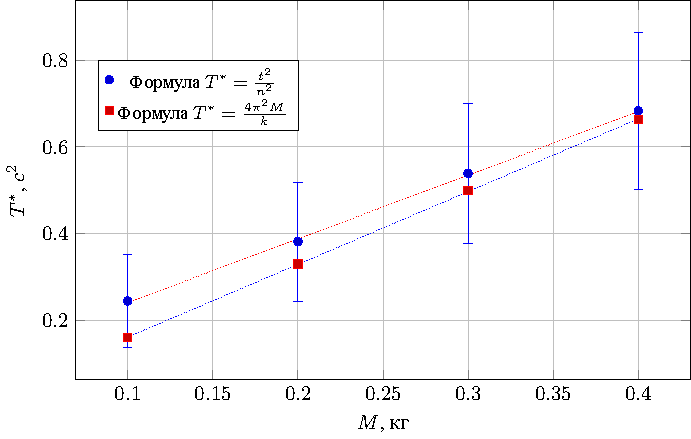
\includegraphics[scale=1.5]{img/graph_3}
	\caption{График зависимости квадрата периода от массы груза большой пружины}
	\label{fig:ris3}
\end{figure}
\begin{figure}[htbp]
	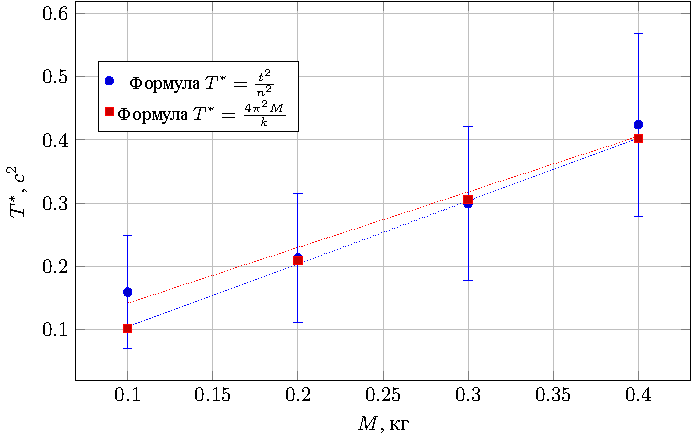
\includegraphics[scale=1.5]{img/graph_4}
	\caption{График зависимости квадрата периода от массы груза малой пружины}
	\label{fig:ris4}
\end{figure}

\newpage
\subsection{Определение зависимости периода колебаний от амплитуды}
Устанавливаем на стенд пружинки с массой груза $M = 300$ г, амплитудой $A$. Начинаем измерения, фиксируя время $n$ полных колебаний. После получения данных, по формуле \ref{eqution: 10} вычисляем период колебаний. (Таблица \ref{tabular:measuring_2})

\begin{table}[htbp]
	\label{tabular:measuring_2}
	\caption{Исследование зависимости периода от амплитуды}
	\centering
	\begin{tabular}{|l|c|c|c|c|c|c|}
		\hline
		          & \multicolumn{3}{c|}{Пружина большая} & \multicolumn{3}{c|}{Пружинка малая} \\ \hline
		Амплитуда & малая & средняя &      большая       & малая & средняя &      большая      \\ \hline
		$A$, см   &  0,5  &    2    &         4          &  0,5  &    2    &         4         \\ \hline
		$n$       &  10   &   10    &         10         &  10   &   10    &        10         \\ \hline
		$t$, с    &  7,6  &   7,4   &        7,2         &  5,3  &   5,2   &        5,1        \\ \hline
		$T$, c    & 0,76  &  0,74   &        0,72        & 0,53  &  0,52   &       0,51        \\ \hline
	\end{tabular}
\end{table}

Вычислим абсолютную погрешность секундомера (Формула \ref{eqution: 20}), т.к. было произведено только одно измерение при разных амплитудах, то будем считать $\triangle t_\text{сл} = 0$, поэтому $\triangle t_\text{пр} = \triangle t$,  и косвенную погрешность периода $T$ (Формула \ref{eqution: 11}, Приложение - \ref{appendix: 11}).

\begin{equation}
	\label{eqution: 21}
	\triangle t = t_{\alpha, \infty} * \frac{\delta _t}{3} = 1,96 * \frac{0,5 \text{ с}}{3} = 0,33 \text{ с}
\end{equation}
\begin{equation}
	\label{eqution: 22}
	\triangle T = \frac{0,33 c}{10} = 0,03 c
\end{equation}

\begin{figure}[htbp]
	\centering
	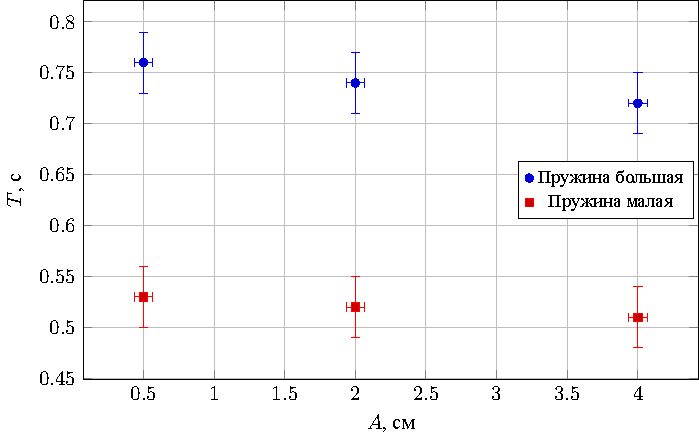
\includegraphics[scale=1]{img/graph_1}
	\caption{График зависимости периода колебаний от амплитуды}
	\label{fig:ris2}
\end{figure}
\newpage
\subsection{Изучение зависимости периода колебаний от времени}
Изучим зависимость периода колебаний от времени. Для этого установим маятник на $A = 4 \text{ см}$, $M = 300 \text{ г}$ и будем фиксировать таймер в моментах, когда амплитуда будет равно отношениям $\frac{3}{4} A_0 = 3 \text{ см}$, $\frac{1}{2} A_0 = 2 \text{ см}$, $\frac{1}{4} A_0 = 1 \text{ см}$. 

\begin{table}[htbp]
	\label{tabular:measuring_4}
	\caption{Исследование зависимости амплитуды колебаний от времени}
	\centering
	\begin{tabular}{|l|c|c|c|c|c|c|}
		\hline
		                                 & № опыта &         $A$, см         &   1   &   2   &   3   &   4   \\ \hline
		\multirow{3}{*}{Пружина большая} &    1    & \multirow{3}{*}{$t$, c} & 0 & 70 & 183 & 545 \\
		                                 &    2    &                         & 0 & 56 & 180 & 515 \\
		                                 &    3    &                         & 0 & 108 & 238 & 555 \\ \hline
		\multirow{3}{*}{Пружинка малая}  &    1    & \multirow{3}{*}{$t$, c} & 0 & 10 & 20 & 69 \\
		                                 &    2    &                         & 0 & 10 & 20 & 55 \\
		                                 &    3    &                         & 0 & 9 & 20 & 55 \\ \hline
	\end{tabular}
\end{table}

Вычислим абсолютную погрешность времени (Формулы \ref{eqution: 20}-\ref{equation: 10}, Приложение \ref{appendix: 4}, \ref{appendix: 12}-\ref{appendix: 14}).

\begin{table}[H]
	\label{tabular:measuring_5}
	\caption{Вычисление абсолютной погрешности t}
	\centering
	\begin{tabular}{|l|c|c|c|}
		\hline
		$S_t,\text{ с}$ & $\triangle t_{\text{ сл}},\text{ с}$ & $\triangle t_{\text{ пр}},\text{ с}$ & $\triangle t, \text{ с}$ \\
		\hline
		0,00 & 0,00 & 0,33 & 0,33 \\
		\hline
		6,34 & 21,28 & 0,33 & 21,28 \\
		\hline
		7,70 & 25,82 & 0,33 & 25,28 \\
		\hline
		4,91 & 16,46 & 0,33 & 16,46 \\
		\hline
		0,00 & 0,00 & 0,33 & 0,33 \\
		\hline
		0,14 & 0,46 & 0,33 & 0,56 \\
		\hline
		0,27 & 0,91 & 0,33 & 0,97 \\
		\hline
		1,91 & 6,39 & 0,33 & 6,40 \\
		\hline
	\end{tabular}
\end{table}
 
\newpage
\begin{figure}[H]
	\centering
	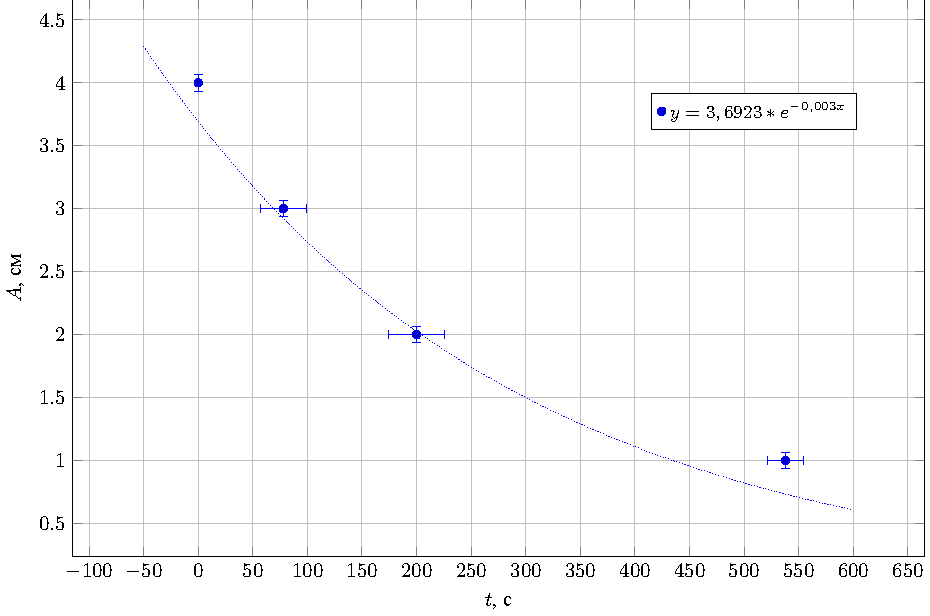
\includegraphics[scale=1]{img/graph_5}
	\caption{График периода колебаний от времени большой пружины}
	\label{fig:ris3}
\end{figure}
\begin{figure}[H]
	\centering
	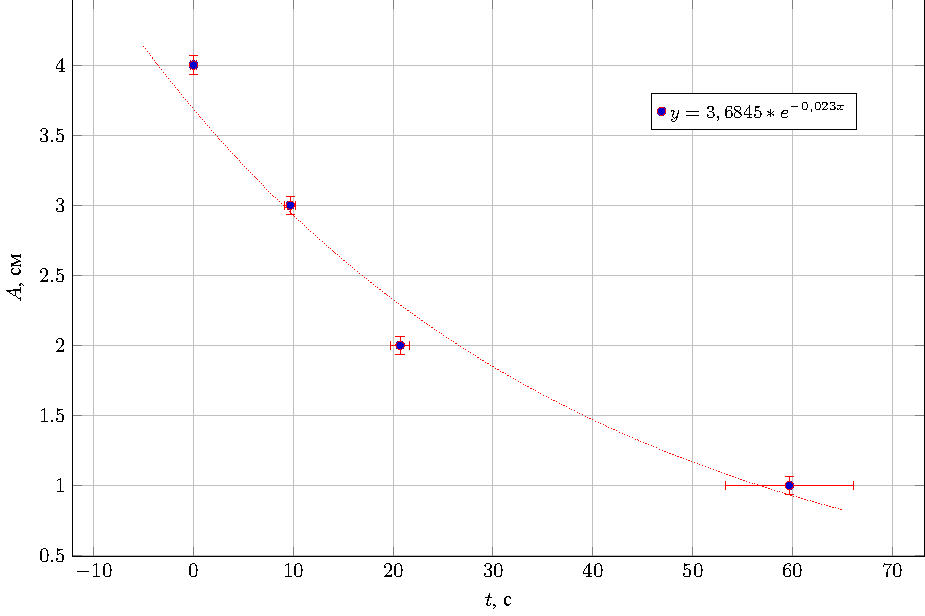
\includegraphics[scale=1]{img/graph_6}
	\caption{График периода колебаний от времени малой пружины}
	\label{fig:ris4}
\end{figure}
 





